\chapter[]{Exploratory Test Results}
\label{app:explo_result}
The results of the initial exploratory performance test, is presented below. This test was conducted initially, in order to get a feel of the execution time for the concurrency model.

\begin{table}[h]
\centering
\begin{tabular}{l|cll|cll}
             & \multicolumn{3}{c|}{Milliseconds} & \multicolumn{3}{c}{Normalized} \\
Iterations Tasks & TL     & STM     & Actor     & TL      & STM      & Actor     \\ \hline
1  	&		2019		&      2017		&		2027    &  1.00   & 1.00 &    1.00    \\
10	&		19290		&      19319		&		19378   &  1.00   & 1.00 &    1.00    \\
20	&		38312		&      38328		&		38390   &  1.00   & 1.00 &    1.00    \\
30	&		57537		&      57508		&		57578   &  1.00   & 1.00 &    1.00    \\
40	&		76701		&      76480		&		76877   &  1.00   & 1.00 &    1.01    \\
50	&		96235		&      95854 	&		96398   &  1.00   & 1.00 &    1.01    \\
60  	&		115203	&      114832	&		115575  &  1.00   & 1.00 &    1.01    \\
70	&		134404	&      133984	&		134495  &  1.00   & 1.00 &    1.00    \\
80	&		153350	&      153082	&		153730  &  1.00   & 1.00 &    1.00    \\
90	&		172521	&      172041	&		172925  &  1.00   & 1.00 &    1.01    \\
100	&		191413	&      190996	&		191914  &  1.00   & 1.00 &    1.00    \\
\end{tabular}
\captionof{table}{Test results for scaling number of mapper iterations}\label{table:test_results_concurrent_tasks}
\end{table}
\label{table:test_results_iterations}

\begin{figure}[h]
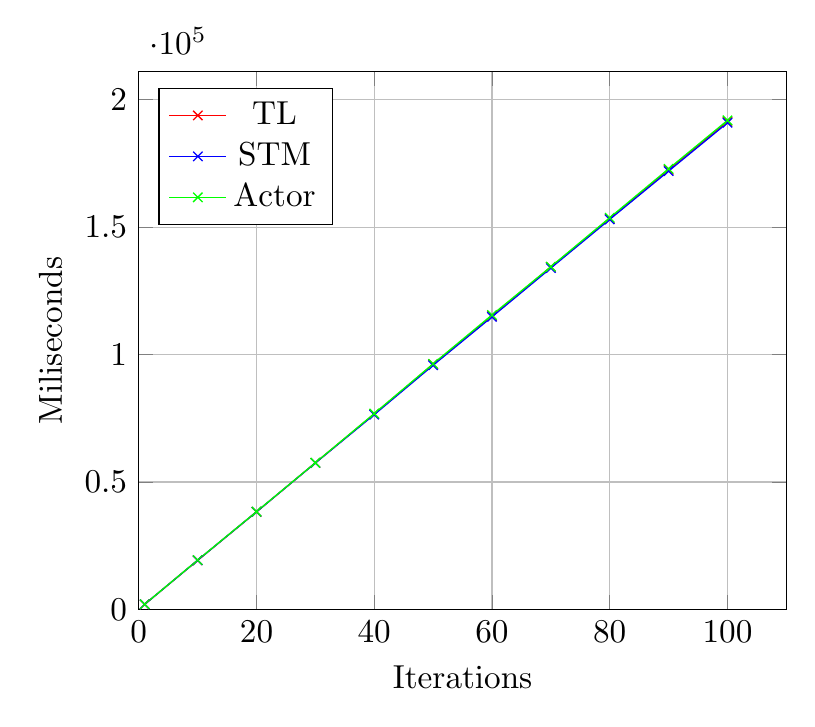
\begin{tikzpicture}[scale=1.2]
	\begin{axis}[
		legend entries={\acs{TL},\acs{STM}, Actor},
		legend pos=north west,
		grid = both,
		xlabel=Iterations,
		ylabel=Miliseconds,
		xmin=0,
		ymin=0,
		label=fig:tr_scale_iterations]		
	\addplot[color=red,mark=x] coordinates {
		(1,2019)
		(10,19290)
		(20,38312)
		(30,57537)
		(40,76701)
		(50,96235)
		(60,115203)
		(70,134404)
		(80,153350)
		(90,172521)
		(100,191413)
	};
	\addplot[color=blue,mark=x] coordinates {
		(1,2017)
		(10,19319)
		(20,38328)
		(30,57508)
		(40,76480)
		(50,95854)
		(60,114832)
		(70,133984)
		(80,153082)
		(90,172041)
		(100,190996)
	};
	\addplot[color=green,mark=x] coordinates {
		(1,2027)
		(10,19378)
		(20,38390)
		(30,57578)
		(40,76877)
		(50,96398)
		(60,115575)
		(70,134495)
		(80,153730)
		(90,172925)
		(100,191914)
	};
	\end{axis}
\end{tikzpicture}
\caption{Visual representation of results for scaling number of iterations}\label{fig:test_results_concurrent_tasks}
\end{figure}